\subsection{Использование палитры компонентов}
\label{sec:manual:pallet_manual}

Внешний вид компонента инспектора свойств показан на рисунке~\ref{sec:manual:components_pallet}.

Во вкладке <<All>> можно найти все предоставляемые в использование виды виджетов:
\begin{itemize}
  \item простые компоненты (Components);
  \item лэйауты (Layouts), представляющие собой компоненты-конейтеры для простых компонентов;
  \item пользовательские шаблоны (Custom templates).
\end{itemize}

\begin{figure}[ht]
  \centering
    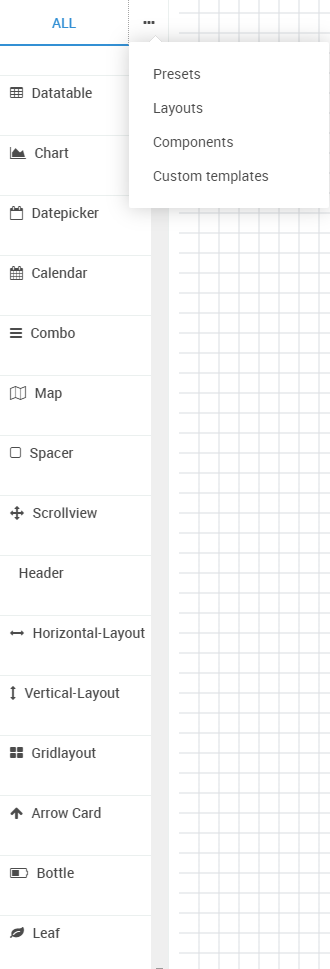
\includegraphics[scale=0.5]{design_components_pallet.png}
    \caption{Внешний вид палитры компонентов}
    \label{sec:manual:components_pallet}
\end{figure}

Список компонентов может содержать более одной колонки компонентов, если ему хватает ширины для того, чтобы все было отрисовано.

Каждому компоненту соответсвует иконка, что облегчает навигацию в списке.\pagebreak

Выбор определенной вкладки осуществляет фильтрацию данных, предоставляемых списком доступных компонентов, по типу компонента, как показано на рисунке~\ref{sec:manual:components_pallet_layouts}.

\begin{figure}[ht]
  \centering
    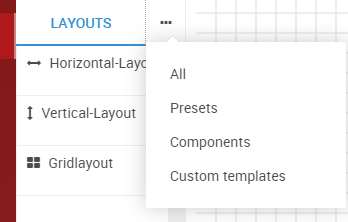
\includegraphics[scale=0.5]{manual_components_pallet(layouts).png}
    \caption{Результат фильтрации списка палитры компонентов}
    \label{sec:manual:components_pallet_layouts}
\end{figure}

